% !TEX root = SegwayDoku.tex
\newpage
\renewcommand{\autoren}{Valentyn Chepil}

\section{Die Hinderniserkennung}
\subsection{Ultraschallsensor}
% \ref{bild_3} zuweisung auf Bild in Text.

\begin{figure}[!h]  % [h] bedeutet, dass das Bild genau an dieser Stelle im Text erscheint
	% mit width=... wird die Größe des Bildes in Prozent der Seitenbreite eingestellt
	\centering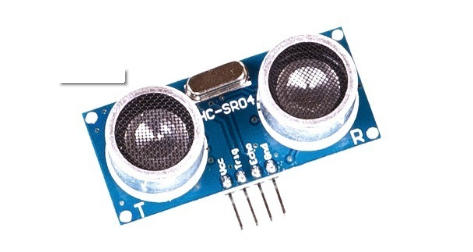
\includegraphics[width=0.5\textwidth]{images/Bild-1-1.png}
	% caption ist die Bildunterschrift, taucht auch im Abbildungsverzeichnis auf
	\caption{Ultraschallsensor \newline(Quelle: funduinoshop.com)}
	\label{bild_1.1} % über das label kann man aus dem Text auf das Bild verweisen
\end{figure}

Die Hinderniserkennung erfolgt über ausgehende Schallwellen, die sich in kegelförmiger Form  ausbreiten. Bei Erreichung des Hindernisses werden die reflektierende Schallwellen aufgenommen und deren Reflektionszeit wird gemessen. Die Ausbreitung und die reflektierenden Schallwellen hängen von verschiedenen Faktoren ab. Sie werden vom Luftdruck, der Umgebungstemperatur, der Luftfeuchtigkeit, sowie vom Sende-/Empfangswinkel und der Oberfläche des im Schallkegel befindlichen Objekts beeinflusst.


\begin{figure}[!h]  % [h] bedeutet, dass das Bild genau an dieser Stelle im Text erscheint
	\centering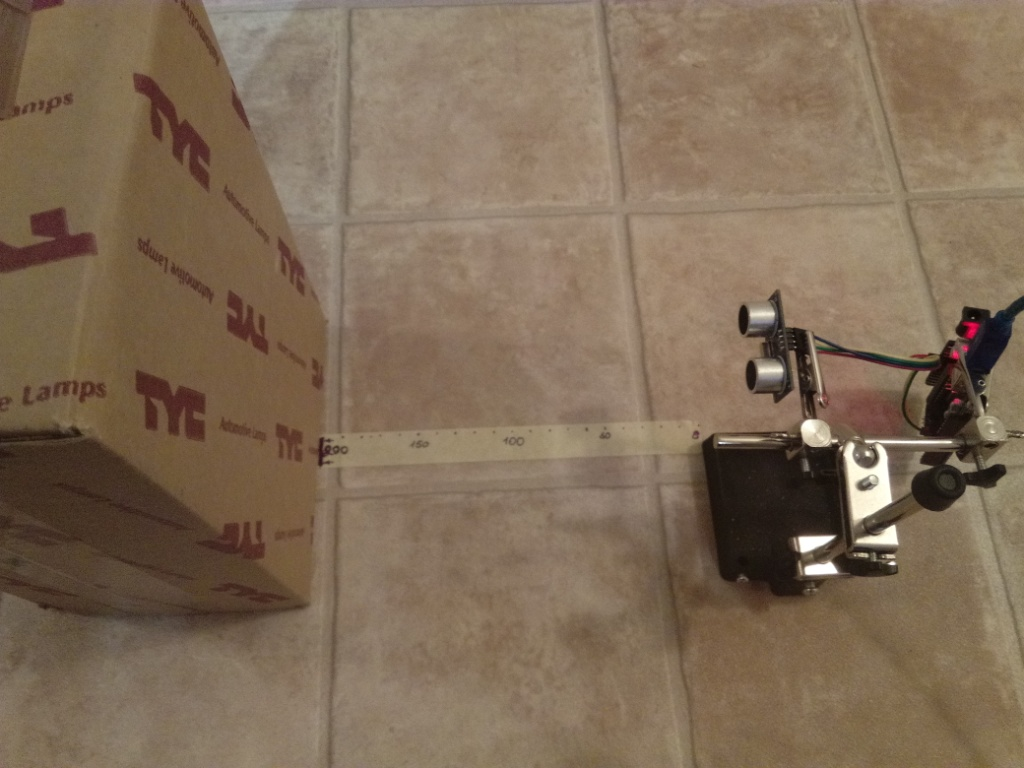
\includegraphics[width=0.6\textwidth]{images/Bild-1.jpg}
	\caption{Entfernungsmessung \newline (Quelle: eigene Darstellung, US-Sensor Messvorgang)}
	\label{bild_1} % über das label kann man aus dem Text auf das Bild verweisen
\end{figure}

\textbf{Vorteile:}  %fett 

Der größte Vorteil der Ultraschallsensoren ist deren günstiger Preis. Dies ermöglicht die Verwendung von vielen Sensoren und somit eine präzise Erfassung der Entfernung zu den Hindernissen. Die Abbildung \ref{bild_1} stellt ein Versuchsaufbau der Hinderniserkennung dar.

\par\bigskip %leere zeile
\textbf{Nachteile:}  %fett 

Ein Hindernis bzw. Objekt kann nicht genau geortet werden, sondern man kann nur feststellen, ob es sich in der gemessenen Entfernung innerhalb des Schallkegels befindet.  Dies ist in der Abbildung \ref{bild_2} zu sehen.

\begin{figure}[ht]  % [h] bedeutet, dass das Bild genau an dieser Stelle im Text erscheint
	\centering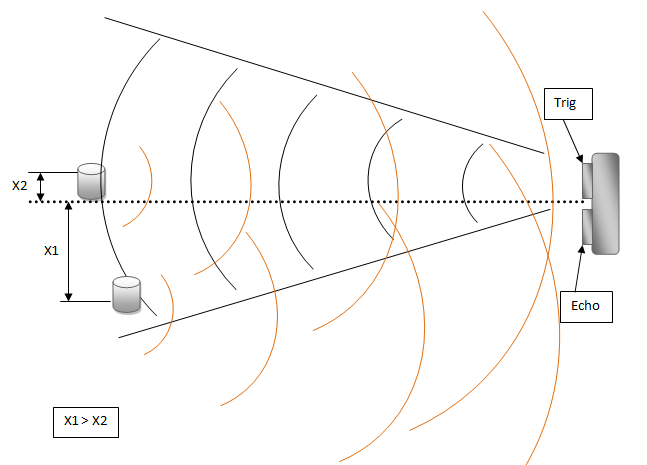
\includegraphics[width=0.6\textwidth]{images/Bild-2.png}
	\caption{Positionierung im Messbereich \newline (Quelle: eigene Darstellung)}
	\label{bild_2} % über das label kann man aus dem Text auf das Bild verweisen
\end{figure}

Bei mehreren Objekten innerhalb einer Schallwelle wird nur der Abstand zum am nächsten liegenden Hindernis gemessen. Die entfernter positionierten Objekte werden nicht erkannt. Das ist in der Abbildung \ref{bild_3} zu sehen.

\begin{figure}[ht]  % [h] bedeutet, dass das Bild genau an dieser Stelle im Text erscheint
	\centering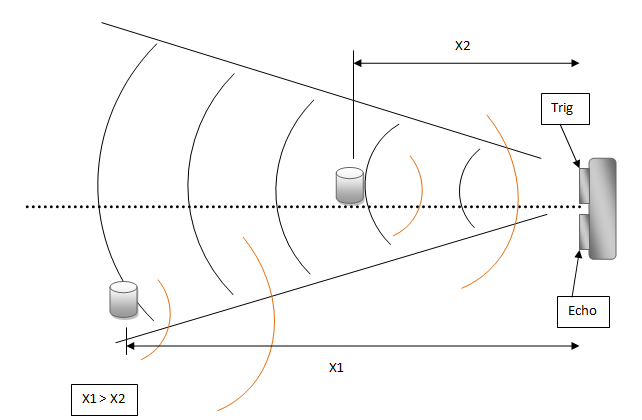
\includegraphics[width=0.6\textwidth]{images/Bild-3.png}
	\caption{Positionierung in Messbereich \newline (Quelle: eigene Darstellung)}
	\label{bild_3} % über das label kann man aus dem Text auf das Bild verweisen
\end{figure}

Nachteilig ist die geringe Reichweite (ca. 3m) des Ultraschalls und  die geringe Ausbreitungsgeschwindigkeit des Schalls, welche bei sich bewegenden Maschinen zur Kollision mit dem Hindernis führen kann.

Große Probleme treten bei den Reflektionseigenschaften der Schallwellen auf. Besonders weichen Materialien und spitzförmigen Oberflächen erkennt  der Sensor schleicht. Ein Beispiel der Oberflächen kann man in der Abbildung \ref{bild_4} und \ref{bild_6} betrachten.

\begin{figure}[!h]  % [h] bedeutet, dass das Bild genau an dieser Stelle im Text erscheint
	\centering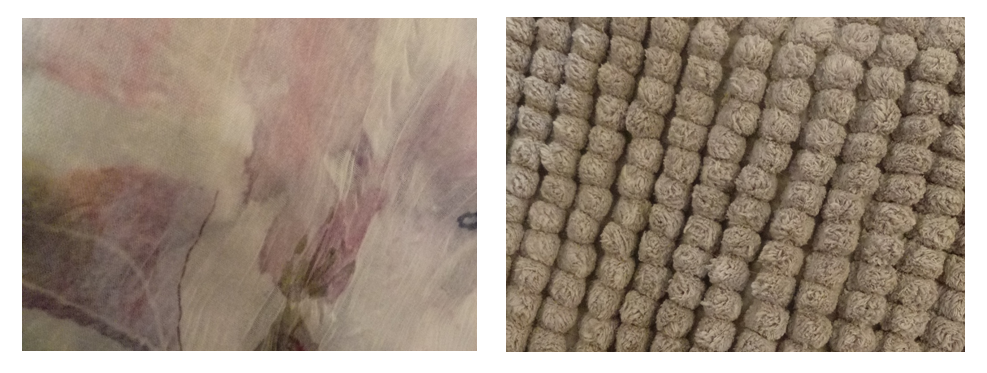
\includegraphics[width=0.7\textwidth]{images/Bild-4-5.png}
	\caption{Weiche und spitzförmig-weiche Oberflächen \newline(Quelle: eigene Darstellung,Frauen-Halsschal und Teppich)}
	\label{bild_4}
\end{figure}
\begin{figure}[!h]  % [h] bedeutet, dass das Bild genau an dieser Stelle im Text erscheint
	\centering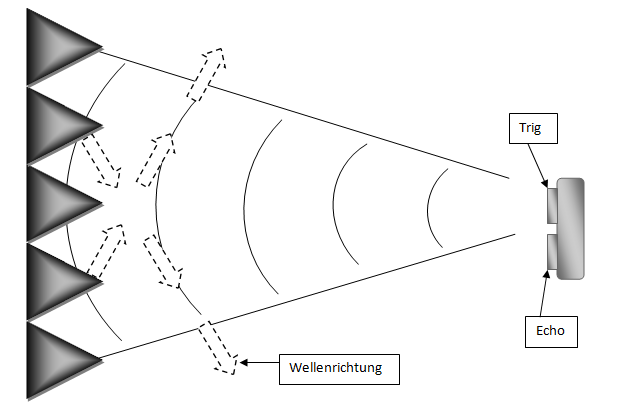
\includegraphics[width=0.6\textwidth]{images/Bild-6.png}
	\caption{Spitzförmige Oberflächen\newline(Quelle: eigene Darstellung, z.B: Kanten)}
	\label{bild_6}
\end{figure}

Wird der Öffnungswinkel des Hindernisses kleiner als 75 Grad, so erreicht die Reflektion den aussendenden Sensor nicht (Bild \ref{bild_7}). 

\begin{figure}[!h]  % [h] bedeutet, dass das Bild genau an dieser Stelle im Text erscheint
	\centering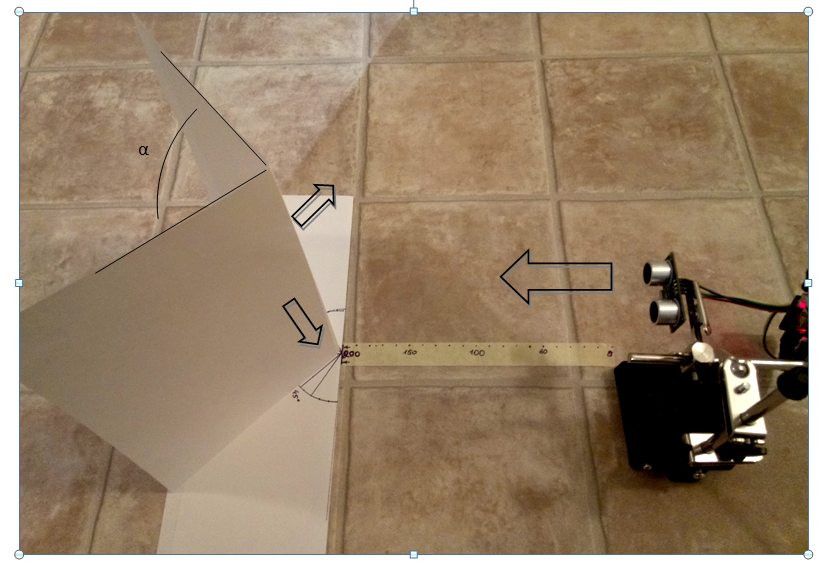
\includegraphics[width=0.6\textwidth]{images/Bild-7.png}
	\caption{Öffnungswinkel (Quelle: eigene Darstellung)}
	\label{bild_7} % über das label kann man aus dem Text auf das Bild verweisen
\end{figure}

Mit den Fähigkeiten des Sensors wurde folgendes Modul konstruiert und angepasst. Auf der Abbildung \ref{H-Mod} ist der Öffnungswinkel von drei US-Sensoren zu sehen.

\begin{figure}[!h]  % [h] bedeutet, dass das Bild genau an dieser Stelle im Text erscheint
	\centering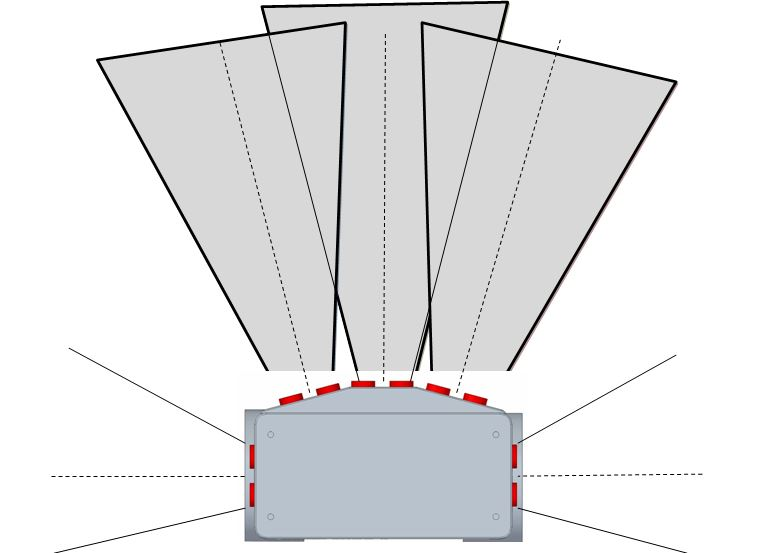
\includegraphics[width=0.95\textwidth]{images/H-Mod.jpg}
	\caption{Modul zur Hinderniserkennung mit Ultraschallsensoren (US1, US2, US22, US3, US33); mit US1 - Mitte, US2, US3 - rechte Seite und US22, US33 - linke Seite  (Quelle: eigene Darstellung)}
	\label{H-Mod} 
\end{figure}

\subsection{Infrarot}
Als Alternative kann man Infrarot-Sensor zusammen mit Ultraschallsensor verwenden, da der Sensor höhere Reaktionszeit hat. Den Sensor kann man auf dem  Bild \ref{infrarot} betrachten.

\begin{figure}[!h]  % [h] bedeutet, dass das Bild genau an dieser Stelle im Text erscheint
	\centering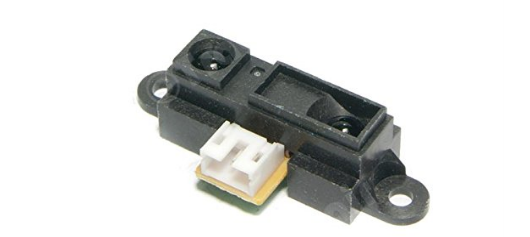
\includegraphics[width=0.6\textwidth]{images/infrarot.png}
	\caption{ \ Infrarot-Sensor  (Quelle: amazon.de)}
	\label{infrarot} % über das label kann man aus dem Text auf das Bild verweisen
\end{figure}
\pagebreak
